\chapter{Introduction}

- deepfake is buzzword (no agreed-upon technical definition)
- ...

\chapter{Deepfakes}

The creation of fake media and their detection have been a problem since photography was invented. Digital photography or video with tools such as GIMP, Adobe Photoshop or Adobe After Effects allows more people to create fakes than before, still some experience in this area is needed. Media that have been modified or otherwise manipulated are called synthetic media, and they do not depend on whether it is an analogue or digital medium. Deepfakes also fall under this category \cite{IncreasingThreatofDeepfakeIdentites}. Tools powered by deep learning allow unexperienced users to easily create trusted fakes. 

The quality of deepfakes reached a level when a trained person or even an experienced researcher in this field has a problem of spotting them. This fast development allows creating realistically looking assets to art photography or movie production, unfortunately, it can be used for malicious purposes like creating fake porn videos to blackmail people or manipulate public via fake news. There are many use cases where deepfakes can be applied.

It is putting huge pressure on researchers to develop new forensics tools or any technology which will prevent malicious usage of deepfakes. As mentioned before, creating fakes is not new, and a whole field of study engaged in spotting fakes and developing techniques over 15 years. Despite continuous research efforts in the past, the advent of deep learning changed the rules of the game. \cite{MediaForensicsandDeepFakes}

\section{Human capabilities of deepfake detection}

The human ability to recognize fake materials from the originals is in contradiction to their quality. Korshunov and Marcel confirmed this in their research. They created a questionnaire containing several videos and the subject (interviewee) had to answer after watching the video whether the person in the video was genuine, fake or they are uncertain. The videos were manually divided into five categories (very easy, easy, moderate, difficult, and very difficult, original). 

Videos were split into several categories manually by researchers probably without usage of any metrics but based on their personal feelings, and ANOVA test shows there is an overlap in several categories so several videos could be moved to different category. However, the categories are still significantly different. 

The results of test in figure \ref{fig:subjective_answers} certainly demonstrate that people's recognition ability decreases significantly as the quality of deepfakes increases. Also, audience of this test knows they are looking for fakes, otherwise we can expect worse results if there will be unsuspected audience (for example: deepfakes on social media). It is quite alarming that the correct answers in the category of “very easy” reach only 71,1 \%. The quality of deepfake increases over time, thus it can be expected that human recognition ability will continue to decrease. \cite{TheThreatOfDeepfakes}

\begin{figure*}[ht]
    \begin{subfigure}[h]{.45\linewidth}
        \centering
        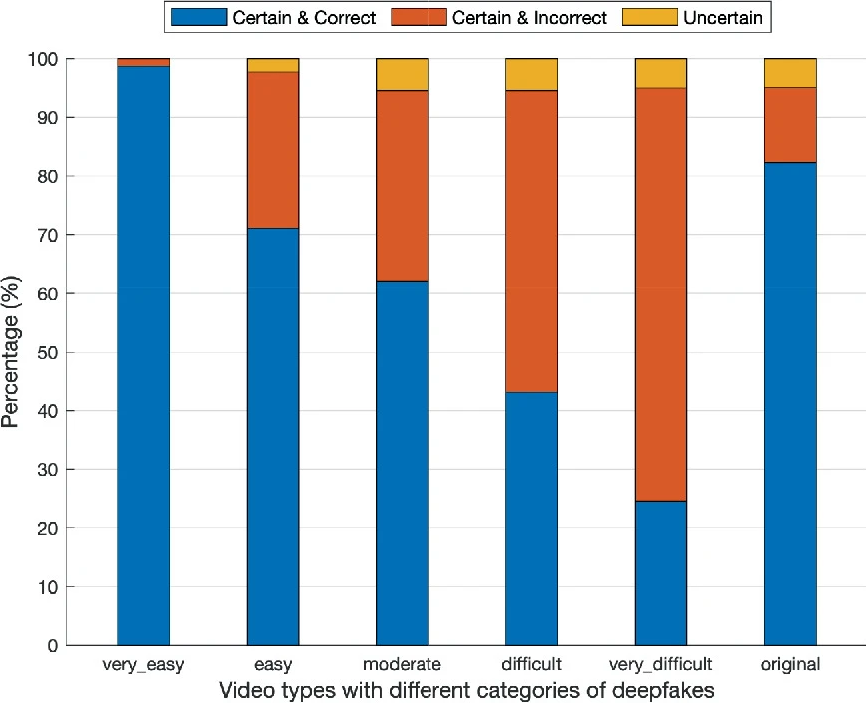
\includegraphics[width=1\linewidth]{other-fig/subjective_answers_a.png}
        \caption{Subjective answers}
    \end{subfigure}
    \hfill
    \begin{subfigure}[h]{.45\linewidth}
        \centering
        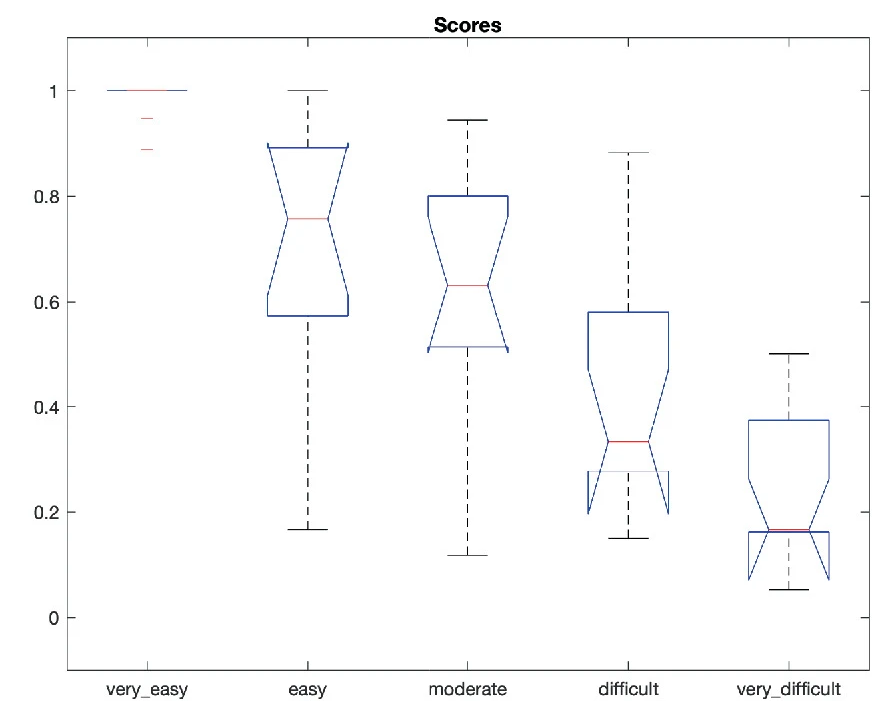
\includegraphics[width=1\linewidth]{other-fig/subjective_answers_b.png}
        \caption{ANOVA test}
    \end{subfigure}
    \caption{Subjective answers and median values with error bars from ANOVA test for different deepfake categories \cite{TheThreatOfDeepfakes}.}
    \label{fig:subjective_answers}
\end{figure*}

Another research tested only recognition of audio tracks and they were comparing humans versus computer programs. Attendees had correct classification between fakes and origins 67 \% after the first several rounds. Their accuracy increased while listening and answering to more tracks, but the value stabilizes on 80 \%. On average trained AI performs about 10 \% better than human, but this result highly depends on difference of learning and test dataset. Still, it shows that the computer can outperform humans in spotting deepfakes. \cite{HumanPerceptionAudio}

\section{Potentional risks}

\cite{DawnOfTextDependentSociety}
\cite{IncreasingThreatofDeepfakeIdentites}

\section{Types of deepfakes and their generation}

\chapter{Analysis of existing tools for detecting deepfakes}
\section{A}
\section{B}
\section{C}

\chapter{Deepfake detection}
\section{Voice deepfakce detection}
\section{Image/Video deepfakce detection}
\section{A}
\section{B}
\section{C}

\chapter{Architecture analysis}


\chapter{Framework architecture}
\section{High level architecture}
\section{Containerazation and scaling}
\section{Input layer}
\section{Data preparation layer}
\section{Inividual detection containers}

\chapter{Client architecture}
\section{Web plugin}

\chapter{Framework implementation}

\chapter{Client implementation}

\chapter{Test experiment and results}

\chapter{Conclusion}